\documentclass{beamer}
\usepackage{../common_slides}
\usepackage{tikz-qtree}
\usepackage{listings}
\usepackage{stackengine}
\stackMath
\newlength\matfield
\newlength\tmplength
\def\matscale{1.}
\newcommand\dimbox[3]{%
  \setlength\matfield{\matscale\baselineskip}%
  \setbox0=\hbox{\vphantom{X}\smash{#3}}%
  \setlength{\tmplength}{#1\matfield-\ht0-\dp0}%
  \fboxrule=1pt\fboxsep=-\fboxrule\relax%
  \fbox{\makebox[#2\matfield]{\addstackgap[.5\tmplength]{\box0}}}%
}
\newcommand\raiserows[2]{%
   \setlength\matfield{\matscale\baselineskip}%
   \raisebox{#1\matfield}{#2}%
}
\newcommand\matbox[4]{
  \stackunder{\dimbox{#1}{#2}{$#4$}}{\scriptstyle #3}%
}

\title{Part-of-Speech Tagging \\ + \\ Neural Networks}
\date{}
\author{CS 287}
\begin{document}


\begin{frame}
  \titlepage
\end{frame}


\begin{frame}{Quiz}
  Last class we focused on hinge loss.

  \[L_{hinge} = \max\{0, 1 - (\hat{y}_c - \hat{y}_{c'}) \} \]

  Consider now the squared hinge loss, (also called $\ell_2$ SVM)

  \[L_{hinge^2} = \max\{0, 1 - (\hat{y}_c - \hat{y}_{c'}) \}^2 \]

  What is the effect does this have on the loss?
  How do the parameters gradients change?
\end{frame}



\section{Part-of-Speech Data}

\begin{frame}{Penn Treebank (Marcus et al, 1993)}

\lstset{ basicstyle=\ttfamily, breaklines=true}

\texttt{
( (S (CC But)
    (SBAR-ADV (IN while)
      (S
        (NP-SBJ (DT the) (NNP New) (NNP York) (NNP Stock) (NNP Exchange) )
        (VP (VBD did) (RB n't)
          (VP (VB fall)
            (ADVP-CLR (RB apart) )
            (NP-TMP (NNP Friday) )
            (SBAR-TMP (IN as)
              (S
                (NP-SBJ (DT the) (NNP Dow)
                (NNP Jones) (NNP Industrial) (NNP Average) )
                (VP (VBD plunged)
                  (NP-EXT
                    (NP (CD 190.58) (NNS points) )
                    (PRN (: -)
                      (NP
                        (NP (JJS most) )
                        (PP (IN of)
                          (NP (PRP it) ))
                        (PP-TMP (IN in)
                          (NP (DT the) (JJ final) (NN hour) )))
                      (: -) )))))))))
    (NP-SBJ-2 (PRP it) )
    (ADVP (RB barely) )
    (VP (VBD managed)
      (S
        (NP-SBJ (-NONE- -2) )
        (VP (TO to)
          (VP (VB stay)
            (NP-LOC-PRD
              (NP (DT this) (NN side) )
              (PP (IN of)
                (NP (NN chaos) )))))))
    (. .)))
}
\end{frame}

\begin{frame}{Syntax}
\begin{center}
\scalebox{0.3}{

\Tree [.S [.S  [.NP [.ADJP Battle-tested industrial ]
managers ]
[.? here ]
[.? always ]
[.VP buck ] ]
[.? [.PP up
[.NP nervous newcomers ] ] ]
[.? [.PP with
[.NP the tale
[.PP of
[.NP the
[.ADJP first ] ] ] ] ] ]
[.? [.PP of
[.NP their countrymen ] ] ]
[.? [.S [.NP * ]
to
[.VP visit
[.NP Mexico ] ] ] ]
[.? , ]
[.? [.NP a boatload
[.PP of
[.NP warriors ] ]
[.VP blown
[.? ashore ]
[.NP 375 years ] ] ] ]
[.? ago ]
[.? . ]   ]}
\end{center}

\pause
\begin{center}

\scalebox{0.7} {
\Tree  [.NP a boatload
[.PP of
[.NP warriors ] ]
[.VP blown
[.? ashore ]
[.NP 375 years ] ] ]}
\end{center}
\end{frame}


\begin{frame}{Tagging}
    \begin{quote}
So
what
if
Steinbach
had
struck
just
seven
home
runs
in
130
regular-season
games
,
and
batted
in
the
seventh
position
of
the
A
's
lineup
.
  \end{quote}

\end{frame}


\begin{frame}{Part-of-Speech Tags}

  \begin{quote}
So/RB
what/WP
if/IN
Steinbach/NNP
had/VBD
struck/VBN
just/RB
seven/CD
home/NN
runs/NNS
in/IN
130/CD
regular-season/JJ
games/NNS
,/,
and/CC
batted/VBD
in/IN
the/DT
seventh/JJ
position/NN
of/IN
the/DT
A/NNP
's/NNP
lineup/NN
./.
  \end{quote}

\end{frame}


\begin{frame}{Part-of-Speech Tags}

  \begin{quote}
So/RB
what/WP
if/IN
Steinbach/NNP
had/VBD
struck/VBN
just/RB
seven/CD
home/NN
runs/NNS
in/IN
130/CD
regular-season/JJ
games/NNS
,/,
and/CC
batted/VBD
in/IN
the/DT
seventh/JJ
position/NN
of/IN
the/DT
A/NNP
's/NNP
lineup/NN
./.
  \end{quote}

\end{frame}


\begin{frame}[allowframebreaks,t]{``Simplified'' English Tagset}
  \begin{enumerate}
  \item , Punctuation
  \item CC Coordinating conjunction
  \item CD Cardinal number
  \item DT Determiner
  \item EX Existential there
  \item FW Foreign word
  \item IN Preposition or subordinating conjunction
  \item  JJ Adjective
  \item JJR Adjective, comparative
  \item JJS Adjective, superlative
  \item LS List item marker
  \item MD Modal
  \item NN Noun, singular or mass
  \item NNS Noun, plural
  \item NNP Proper noun, singular
  \item NNPS Proper noun, plural
  \item PDT Predeterminer
  \item POS Possessive ending
  \item PRP Personal pronoun
  \item PRP\$ Possessive pronoun
  \item RB Adverb
  \item RBR Adverb, comparative
  \item RBS Adverb, superlative
  \item RP Particle
  \item SYM Symbol
  \item TO to
  \item UH Interjection
  \item VB Verb, base form
  \item VBD Verb, past tense
  \item VBG Verb, gerund or present participle
  \item VBN Verb, past participle
  \item VBP Verb, non-3rd person singular present
  \item VBZ Verb, 3rd person singular present
  \item WDT Wh-determiner
  \item WP  Wh-pronoun
  \item WP\$ Possessive wh-pronoun
  \item WRB Wh-adverb
  \end{enumerate}
\end{frame}

\begin{frame}


\textbf{NN or NNS}

\begin{quote}
  Whether a noun is tagged singular or plural depends not on its
  semantic properties, but on whether it triggers singular or plural
  agreement on a verb. We illustrate this below for common nouns, but
  the same criterion also applies to proper nouns.

Any noun that triggers singular agreement on a verb should be tagged as singular, even if it ends in final -s.

\air

\textnormal{EXAMPLE: Linguistics NN is/*are a difficult field.}

\air
If a noun is semantically plural or collective, but triggers singular agreement, it should be tagged as
singular.

\air
\textnormal{EXAMPLES: The group/NN has/*have disbanded.}

\textnormal{The jury/NN is/*are deliberating.}

\end{quote}

\end{frame}


\begin{frame}{Language Specific?}
  \begin{itemize}
  \item Which of these tags are English only?
    \air

  \item Are there  phenomenon that these don't cover?
    \air

  \item Should our models be language specific?
  \end{itemize}
\end{frame}

\begin{frame}{Universal Part-of-Speech Tags (Petrov et al, 2012)}

  \begin{enumerate}
  \item VERB - verbs (all tenses and modes)
  \item NOUN - nouns (common and proper)
  \item PRON - pronouns
  \item ADJ - adjectives
  \item ADV - adverbs
  \item ADP - adpositions (prepositions and postpositions)
  \item CONJ - conjunctions
  \item DET - determiners
  \item NUM - cardinal numbers
  \item PRT - particles or other function words
  \item X - other: foreign words, typos, abbreviations
  \item . - punctuation
\end{enumerate}
\end{frame}


\begin{frame}{Why do tags matter?}
  \begin{itemize}
    \item Interesting linguistic question.
      \air

    \item Used for many downstream NLP tasks.
    \air

    \item Benchmark linguistic NLP task.
  \end{itemize}
  \pause

  However note,

  \begin{itemize}
  \item Possibly have ``solved'' PTB tagging (Manning, 2011)
    \air

  \item Deep Learning skepticism
  \end{itemize}
\end{frame}

\section{Part-of-Speech Models}

\begin{frame}{Strawman: Sparse Word-only Tagging Models}
  Let,
  \begin{itemize}
  \item $\mcF$; just be the set of word type
    \air
  \item $\mcC$; be the set of part-of-speech tags, $|\mcC|\approx 40$
    \air
  \item Proposal: Use a linear model, $\hat{y} = f(\boldx \boldW + \boldb)$
  \end{itemize}

\end{frame}


\begin{frame}{Why is tagging hard?}
  \begin{enumerate}
  \item
  Rare Words
  \begin{itemize}
  \item 3\% of tokens in PTB dev are unseen.
  \item What can we even do with these?
  \end{itemize}

  \item Ambiguous Words
  \begin{itemize}
  \item Around 50\% of seen dev tokens are ambiguous in train.
  \item How can we decide between different tags for the same type?
  \end{itemize}
  \end{enumerate}
\end{frame}


\begin{frame}{Better Tag Features: Word Properties}
  Representation can use specific aspects of text.
  \begin{itemize}
  \item $\mcF$; Prefixes, suffixes, hyphens, first capital, all-capital, hasdigits, etc.
  \item $\boldx = \sum_{i} \bolddelta(f_i)$
  \end{itemize}

  Example: Rare word tagging

  \begin{center}
    \texttt{in 130 \alert{regular-season/*} games ,}
  \end{center}
  \begin{eqnarray*}
    \boldx &=& \delta(\texttt{prefix:3:reg}) + \delta(\texttt{prefix:2:re}) \\
    &+& \delta(\texttt{prefix:1:r}) + \delta(\texttt{has-hyphen}) \\
    &+& \delta(\texttt{lower-case}) + \delta(\texttt{suffix:3:son}) \ldots
  \end{eqnarray*}
\end{frame}

\begin{frame}{Better Tag Features: Tag Sequence}
  Representation can use specific aspects of text.
  \begin{itemize}
  \item $\mcF$; Prefixes, suffixes, hyphens, first capital, all-capital, hasdigits, etc.
  \item \structure{Also} include features on previous tags
  \end{itemize}

  Example: Rare word tagging with context

  \begin{center}
    \texttt{in \structure{130/CD} \alert{regular-season/*} games ,}
  \end{center}
  \begin{eqnarray*}
    \boldx &=& \delta(\texttt{last:CD}) + \delta(\texttt{prefix:3:reg}) + \delta(\texttt{prefix:2:re}) \\
    &+& \delta(\texttt{prefix:1:r}) + \delta(\texttt{has-hyphen}) \\
    &+& \delta(\texttt{lower-case}) + \delta(\texttt{suffix:3:son}) \ldots
  \end{eqnarray*}

  \alert{However,} requires search. HMM-style sequence algorithms.
\end{frame}

% \begin{frame}{Modeling Context}
%   \begin{itemize}
%   \item Features on context require inference.
%   \item Still standard way to do tagging.
%   \item Very fast implementation in Stanford CoreNLP
%   \end{itemize}
% \end{frame}

\begin{frame}{NLP (almost) From Scratch (Collobert et al. 2011)}
  Exercise: What if we just used words and context?

  \begin{itemize}
  \item No word-specific features (mostly)
    \air

  \item No search over previous decisions

    \air
  \end{itemize}



  Next couple classes, we will work our way up to this paper,

  \begin{enumerate}
  \item Dense word features
  \item Contextual windowed representations
  \item Neural networks architecture
  \item Semi-supervised training
  \end{enumerate}
\end{frame}


\section{Bilinear Model}

\begin{frame}{Motivation: Dense Features}
  \begin{itemize}
  \item Strawman linear model learns one parameter for each word.
    \air
  \item Features allow us to share information between words.
    \air
  \item Can this be learned?
  \end{itemize}
\end{frame}


\begin{frame}{Bilinear Model}
  Bilinear model,
  \[\hat{\boldy} = f((\boldx^0 \boldW^0)\boldW^1 + \boldb)\]
  \begin{itemize}
  \item $\boldx^0 \in \reals^{1 \times d_0}$ start with one-hot.
  \item $\boldW^0 \in \reals^{d_0 \times \din}$, $d_0 = |\mcF|$
  \item $\boldW^1 \in \reals^{\din \times \dout}, \boldb \in \reals^{1 \times \dout}$; model parameters
  \end{itemize}
  \air
  Notes:
  \begin{itemize}
  \item Bilinear parameter interaction.
  \item $d_0 >> \din$, e.g. $d_0 = 10000, \din = 50$
  \end{itemize}

\end{frame}

\begin{frame}{Bilinear Model: Intuition}
  \[ (\boldx^0 \boldW^0)\boldW^1 + \boldb\]

  \[
    \begin{bmatrix}
      0 & \ldots & \textcolor{red}{1} & \ldots & 0 \\
    \end{bmatrix}
    \begin{bmatrix}
      w^0_{1,1} &  \ldots &w^0_{0, \din}\\
      & \vdots & \\
      & \vdots & \\
      & \vdots & \\
      \textcolor{red}{w^0_{k,1}} &  \textcolor{red}{\ldots} &\textcolor{red}{w^0_{k,\din}}\\
      & \vdots & \\
      & \vdots & \\
      & \vdots & \\
      w^0_{d_0, 1} &  \ldots &w^0_{d_0, \din}\\
    \end{bmatrix}
    \begin{bmatrix}
      \textcolor{red}{w^1_{1,1}} &  \ldots & \ldots &   \textcolor{red}{w^1_{0, \dout}}\\
      & \ddots & \ddots &  \\
      \textcolor{red}{w^1_{\din,0}} &  \ldots & \ldots & \textcolor{red}{w^1_{\din, \dout}}\\
    \end{bmatrix}
  \]

\end{frame}

\begin{frame}{Embedding Layer}
  \[ \boldx^0 \boldW^0\]
  \begin{center}

  \scalebox{0.6}{
  \[ \begin{bmatrix}
      0 & \ldots & \textcolor{red}{1} & \ldots & 0 \\
    \end{bmatrix}
    \begin{bmatrix}
      w^0_{1,1} &  \ldots &w^0_{0, \din}\\
      & \vdots & \\
      & \vdots & \\
      & \vdots & \\
      \textcolor{red}{w^0_{k,1}} &  \textcolor{red}{\ldots} &\textcolor{red}{w^0_{k,\din}}\\
      & \vdots & \\
      & \vdots & \\
      & \vdots & \\
      w^0_{d_0, 1} &  \ldots &w^0_{d_0, \din}\\
    \end{bmatrix}\]}
  \end{center}
  \begin{itemize}
  \item Critical for natural language applications
  \item Informal names for this idea,
    \begin{itemize}
    \item Feature embeddings/ word embeddings
    \item Lookup Table
    \item Feature/Representation Learning
    \item In Torch, \texttt{nn.LookupTable} ($\boldx^0$ one-hot)
    \end{itemize}
  \end{itemize}
\end{frame}

\begin{frame}{Dense Features}
  When dense features implied we will write,
  \[\hat{\boldy} = f(\boldx\boldW^1 + \boldb)\]


  Example 1: single-word classfication with embeddings

  \[ \boldx = v(f_1; \theta) = \bolddelta(f_1) \boldW^0 = \boldx^0 \boldW^0\]

  \begin{itemize}
  \item $v: \mcF \mapsto \reals^{1\times \din}$; parameterized embedding function
  \end{itemize}


  \pause
  \mathbf{Example 2}: Bag-of-words classfication with embeddings

  \[ \boldx = \sum_{i=1}^{k} v(f_i; \theta) = \sum_{i=1}^{k} \bolddelta(f_i) \boldW^0\]
\end{frame}

\begin{frame}{Log-Bilinear Model}


  \[ \hat{\boldy} =  \softmax (\boldx \boldW^1 + \boldb) \]

  \begin{itemize}
  \item Same form as multiclass logistic regression, but with dense features.
  \item However, objective is now non-convex (no restrictions on $\boldW^0$, $\boldW^1$)
  \end{itemize}
\end{frame}

\begin{frame}{Log-Bilinear Model}
  \begin{center}
    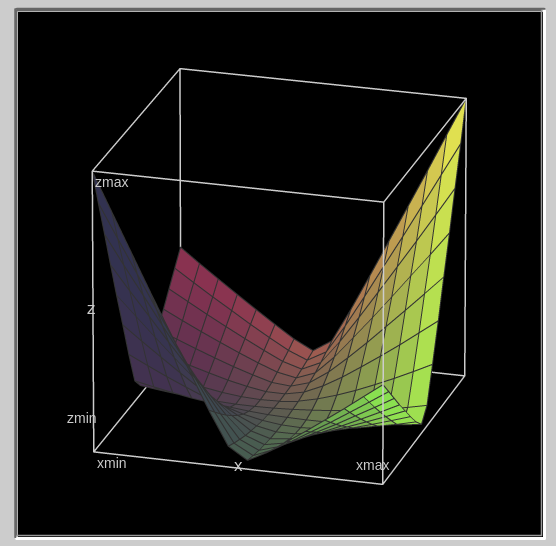
\includegraphics[width=5cm]{logbilinear}
  \end{center}
  \[-15\log \sigma(xy)-5\log\sigma(-xy) + \lambda/2 ||[x\ y]||^2 \]

\end{frame}


\begin{frame}{Does it matter?}
  \begin{itemize}
  \item We are going to use SGD, in theory this is quite bad
    \air
  \item However, in practice it is not that much of an issue
    \air
  \item Argument: in large parameter spaces local optima are okay
    \air
  \item Lots of questions here, beyond scope of class
  \end{itemize}
\end{frame}

\begin{frame}[allowframebreaks]{Embedding Gradients: Cross-Entropy}
  Chain Rule:
  \[ \frac{\partial L(f(\boldx))}{\partial x_i} = \sum_{j =1}^m \frac{\partial f(\boldx)_j} {\partial  x_i} \frac{\partial L(f(\boldx))} {\partial f(\boldx)_j}   \]


  \[ \hat{\boldy} = \softmax (\boldx \boldW^1 + \boldb) \]




  Recall,

  \[ \frac{\partial L(\boldy, \hat{\boldy})}{\partial z_i} =      \begin{cases}
      -(1 - \hat{y}_i) & i = c\\
      \hat{y}_i & ow. \\
    \end{cases} \]



  \[\frac{\partial L}{\partial x_{f}} =
    \sum_{i} W^1_{f, i} \frac{\partial L}{\partial z_{i}} =
     -W^1_{f,c}  (1-\hat{y}_c)  + \sum_{i \neq c} W^1_{f,i}  \hat{y}_i
  \]

  \air
  \air

  \[ \boldx = \boldx^0 \boldW^0 \]

  \[\frac{\partial x_f}{\partial W^0_{k, f'}} = x^0_{k}  \indicator(f = f')   \]

  Update:
  \[\frac{\partial L}{\partial W^0_{k,f'}} = \sum_{f} x^0_{k} \indicator(f = f') \frac{\partial L}{\partial x_{f}}  =  x^0_{k}      (-W^1_{f',c} (1-\hat{y}_c)  + \sum_{i \neq c} W^1_{f',i}  \hat{y}_i)  \]
\end{frame}


% \begin{frame}{Geometric Interpretation}
%   \begin{center}
%     [On Board]
%   \end{center}
% \end{frame}

\section{Windowed Models}


% \begin{frame}{}

% \end{frame}

\begin{frame}{Sentence Tagging}
  \begin{itemize}
  \item $w_1, \ldots, w_n$; sentence words
    \air
  \item $t_1, \ldots, t_n$; sentence tags
    \air

  \item $\mcC$; output class, set of tags.
  \end{itemize}
\end{frame}


\begin{frame}{Window Model}
  \textbf{Goal:} predict $t_5$.


  \begin{itemize}
  \item Windowed word model.

  \[ w_1\ w_2\ [\textcolor{red}{w_3\ w_4\ w_5\ w_6\ w_7}]\ w_8 \]

  \item $w_3, w_4$; left context
  \item $w_5$; Word of interest
  \item $w_6, w_7$; right context

  \item $\dwin$; size of window ($\dwin = 5$)
  \end{itemize}
\end{frame}


\begin{frame}{Boundary Cases}
  \textbf{Goal:} predict $t_2$.
  \[ [\textcolor{red}{ \langle\mathrm{s}\rangle \ w_1\ w_2\ w_3\ w_4}]\ w_5\ w_6\ w_7\ w_8 \]


  \textbf{Goal:} predict $t_8$.
  \[  w_1\ w_2\ w_3\ w_4\ w_5\ [\textcolor{red}{w_6\ w_7\ w_8\  \langle\mathrm{/s}\rangle\ \langle\mathrm{/s}\rangle}] \]

  Here symbols $\langle\mathrm{s}\rangle$ and $\langle\mathrm{/s}\rangle$ represent boundary padding.
\end{frame}


\begin{frame}{Dense Windowed BoW Features }
  \begin{itemize}
  \item $f_1, \ldots, f_{\dwin}$ are words in window
  \item Input representation is the concatenation of embeddings
  \end{itemize}

  \[ \boldx = [v(f_1)\  v(f_2) \  \ldots \  v(f_{\dwin})]  \]

  Example: Tagging
  \[ w_1\ w_2\ [\textcolor{red}{w_3\ w_4\ w_5\ w_6\ w_7}]\ w_8 \]
  \[ \boldx = [v(w_3)\  v(w_4) \  v(w_5) \ v(w_6) \ v(w_7)]  \]

  \[\renewcommand\matscale{.6}
\matbox{1.5}{4}{\din /5}{} \matbox{1.5}{4}{\din /5}{} \matbox{1.5}{4}{\din /5}{\boldx} \matbox{1.5}{4}{\din /5}{} \matbox{1.5}{4}{\din /5}{}% \raiserows{1.5}{\matbox{4}{2}{d_0}{\dout}{\boldW^0}}  \matbox{4}{2}{\din}{\dout}{\boldW^1} +
% \matbox{7}{2}{1}{\dout}{\boldb}
\]

Rows of $\boldW^1$ encode position specific weights.
\end{frame}


\begin{frame}{Dense Windowed Extended Features }
  \begin{itemize}
  \item $f_1, \ldots, f_{\dwin}$ are words, $g_1, \ldots, g_{\dwin}$ are capitalization
  \end{itemize}

  \[ \boldx = [v(f_1)\  v(f_2) \  \ldots \  v(f_{\dwin})\ v_2(g_1)\  v_2(g_2) \  \ldots \  v_2(g_{\dwin})]  \]

  Example: Tagging
  \[ w_1\ w_2\ [\textcolor{red}{w_3\ w_4\ w_5\ w_6\ w_7}]\ w_8 \]
  \[ \boldx = [v(w_3)\  v(w_4) \  v(w_5) \ v(w_6) \ v(w_7) \ v_2(w_3)\  v_2(w_4) \  v_2(w_5) \ v_2(w_6) \ v_2(w_7)]  \]

  \[\renewcommand\matscale{.6}
\matbox{1.5}{4}{}{} \matbox{1.5}{4}{}{} \matbox{1.5}{4}{}{} \matbox{1.5}{4}{}{} \matbox{1.5}{4}{}{\boldx} \matbox{1.5}{2}{}{} \matbox{1.5}{2}{}{} \matbox{1.5}{2}{}{} \matbox{1.5}{2}{}{} \matbox{1.5}{2}{}{}% \raiserows{1.5}{\matbox{4}{2}{d_0}{\dout}{\boldW^0}}  \matbox{4}{2}{\din}{\dout}{\boldW^1} +
% \matbox{7}{2}{1}{\dout}{\boldb}
\]

Rows of $\boldW^1$ encode position/feature specific weights.
\end{frame}


\begin{frame}{Tagging from Scratch (Collobert et al, 2011)}
  Part 1 of the key model,
  \begin{center}
    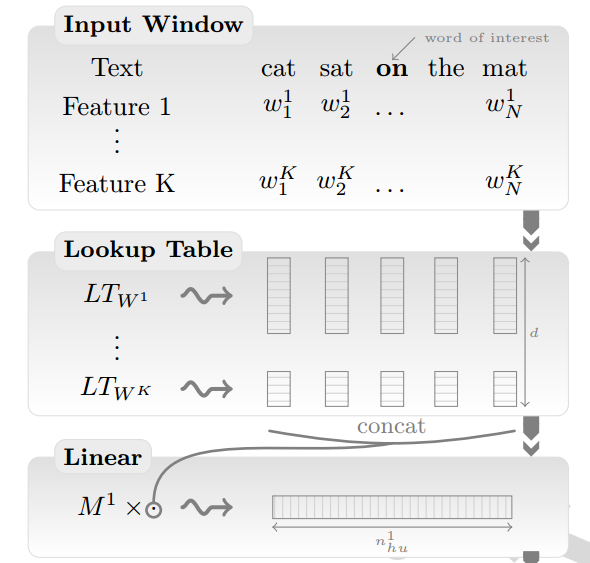
\includegraphics[width=5cm]{cwlin}
  \end{center}
\end{frame}


% \begin{frame}{The Role of Features}
%   \begin{itemize}
%   \item Recall Zipf's law.
%   \item Many words are ..
%   \item Can capture patterns.
%     example.
%   \end{itemize}
% \end{frame}

% \begin{frame}{How much does this matter?}
%   graph of tagging.
% \end{frame}

% \begin{frame}{Sparse Tagging Model}
%   \begin{itemize}
%   \item Create training data,
%     \[ (\boldx_1, \boldy_1),\ldots , (\boldx_n, \boldy_n)\]
%   \item Each $\boldx_i$ includes features of window.
%   \item Each $\boldy_i$ is the one-hot tag encoding.
%   \item Prediction accuracy is measured identically.
%   \end{itemize}
% \end{frame}


% \begin{frame}{Naive Bayes/Logistic Regression for Tagging}
%   \begin{itemize}
%   \item Setup is identical to text classification.

%   \item \[ \hat{\boldy} = \boldx \boldW + \bold b \]
%   \end{itemize}
% \end{frame}

% \section{Neural Networks}

% \begin{frame}
%   Collobert and Weston
%   Natural Language Processing (almost) from Scratch
% \end{frame}

% \begin{frame}{Two ideas}


%   \begin{itemize}
%   \item Non-linear Models
%   \item Dense Word embeddings
%   \end{itemize}
% \end{frame}


% \begin{frame}{(1) Non-Linear Models for Classification}
%   \begin{itemize}
%   \item Neural network represent any non-linear classifier, for example
%     \[ NN_1 = f_1(\boldx \boldW^1 + \boldb^1))  \]
%     \[ \hat{\boldy} = f_2(NN_1 \boldW^2 + \boldb^2)  \]
%   \item Where $\boldW^1 \in \reals^{\din \times dmid}, \boldb^1 \in \reals^{1\times dmid}$
%   \item  $\boldW^2 \in \reals^{dmid \times dout}, \boldb^2 \in \reals^{1\times \dout}$
%   \item Activation $f_1$ is non-linear.

%   \end{itemize}
%   Decision $\argmax \hat{y}$
% \end{frame}

% \begin{frame}{}
%   Can learn non-linear decision boundary.
%   Diagram
% \end{frame}

% \begin{frame}
%   For instance, $f_1$ Sigmoid and $f_2$ softmax

%   \[ \frac{\partial L(y, \hat{y})}{\partial \hat{y}_j} = \frac{\indicator(y_j = 1)} {\hat{y}_j}  \]

% \end{frame}


% \begin{frame}
%   For instance, $f_1$ ReLU and $f_2 $hinge-loss


% \end{frame}


% \begin{frame}{Backpropagation}
%   \begin{itemize}
%   \item Chain rule
%   \end{itemize}
% \end{frame}

% \section{Dense Features}

% \begin{frame}{(2) Dense Features}

%   Instead of defining $\boldx = \sum_{i=1}^n \delta(f_i)$


%   Where $v : \mcF \mapsto \reals^d$ for instance $v(f) = \delta(f) \boldW^0$

%   and define  $\boldx = [ v(f_1) \ldots v(f_k)] $

%   (For now we assume all examples have fixed length)

% \end{frame}

% \begin{frame}{Dense Features for Tagging}

%   Instead of defining $\boldx = \sum_{i=1}^n \delta(f_i)$


%   Where $v : \mcF \mapsto \reals^d$ for instance $v(f) = \delta(f) \boldW^0$

%   and define  $\boldx = [ v(f_1) \ldots v(f_k)] $

%   (For now we assume all examples have fixed length)

% \end{frame}

% \begin{frame}{Dense Features for Tagging}

%   Instead of defining $\boldx = \sum_{i=1}^n \delta(f_i)$


%   Where $v : \mcF \mapsto \reals^d$ for instance $v(f) = \delta(f) \boldW^0$

%   and define  $\boldx = [ v^1(f_1) \ldots v^1(f_k) \ldots v^2(f_k+1) \ldots v^2(f_k)] $

%   (For now we assume all examples have fixed length)

% \end{frame}




% \begin{frame}{Parameters}
%   \begin{itemize}
%   \item With word features $|\mcV|$

%   \item With all pair word features $|\mcV|^2$


%   \item With word embedding features $d |\mcV|$

%     Representation that allows parameter sharing.
%   \end{itemize}
% \end{frame}




% \begin{frame}{Lookup layer is Learned too}
%   results
% \end{frame}

% \begin{frame}
%   Results
%   Pretty good
%   \begin{table}
%     \centering

%   \end{table}
% \end{frame}

% \begin{frame}{}
%   objective

%   Diagram
% \end{frame}



\end{document}
